
\documentclass[journal=nalefd,manuscript=letter]{achemso}

\usepackage{chemformula} 
\usepackage[T1]{fontenc} 
\usepackage{soul, color}
\usepackage{wasysym}
\usepackage{natbib}
\usepackage{mathtools}
\usepackage{subfigure}  
\usepackage{amsmath}
\usepackage{caption}
\usepackage{algorithmicx, algpseudocode, algorithm}  % For pseudocode formatting
\usepackage{soul,color}


\author{Julia Frank}
\email{umfran77@myumanitoba.ca}
\affiliation{Department of Physics \& Astronomy, University of Manitoba, Winnipeg, Canada}

\author{Johan van Lierop}
\email{Johan.van.Lierop@umanitoba.ca}
\affiliation{Department of Physics \& Astronomy, University of Manitoba, Winnipeg, Canada}

\author{Robert L. Stamps}
\email{Robert.Stamps@umanitoba.ca}
\affiliation{Department of Physics \& Astronomy, University of Manitoba, Winnipeg, Canada}


\title{\emph{Supporting Information: ReplicaSim} \protect\\ Monopole current control in artificial spin ice via localized fields} 

\keywords{artificial spin ice, nanomagnet, hysteresis, magnetization dynamics, Monte Carlo, control, guided monopole current}

\begin{document}

\newpage

\section{Multi-Replica Parallel GPU-Accelerated\\
Monte Carlo Algorithm}
ReplicaSim employs a standard single-spin-flip Metropolis Monte Carlo algorithm optimized for large-scale ASI simulations using dumbell model for computing dipolar interactions. All computations use single-precision floats (Float32), which provide a good balance between performance and accuracy for our purposes. Below, we outline the key features and implementation details that distinguish ReplicaSim from conventional approaches.

\subsection{Parallel Replica Simulation}
Unlike conventional ASI Monte Carlo methods that simulate one system per run, ReplicaSim evolves up to 1000 independent replicas simultaneously on the GPU. In practice, using on the order of 100 replicas is usually sufficient to obtain good statistical averages and to illustrate the variability introduced by random spin-flip sequences.

For very large spin lattices (where each replica has more than 256 spins), ReplicaSim partitions each replica’s workload across multiple thread blocks on the GPU. In other words, a two-dimensional CUDA grid is launched: one grid dimension indexes the replicas, and the other splits the spins of each replica across several blocks. This ensures that even if a single replica contains thousands of spins (exceeding the threads available in one block), all spins are updated in parallel by distributing them over multiple blocks. This multi-block-per-replica strategy maintains high occupancy and performance for large-scale simulations.

\subsection{CUDA-Accelerated Energy and Magnetization Calculations}
To speed up energy calculations, ReplicaSim uses precomputed neighbor lists and compressed interaction matrices for the dipolar interactions. A compressed interaction matrix stores only the nonzero coupling coefficients for each spin’s nearby neighbours (up to the cutoff distance) rather than a full dense $N \times N$ interaction matrix. In our implementation, four such matrices (denoted $J_{LL}$, $J_{RR}$, $J_{LR}$, $J_{RL}$) are precomputed to account for the pairwise contributions of the dumbbell model’s magnetic charges. Each row in these $J$ matrices corresponds to a given spin and contains the interaction strengths between that spin and each of its neighbours (including any interactions with control elements). By storing interactions in this compact form, we avoid redundant computations during simulation and significantly reduce memory usage and memory access overhead.
Both energy and magnetization computations are fully accelerated on the GPU. 

We implemented a custom parallel reduction kernel for calculating the total magnetization of each replica, which is necessary due to the multi-block distribution of spins per replica. This custom reduction accumulates partial magnetization results from multiple thread blocks and uses fast shared memory and atomic operations to produce the final magnetization per replica. We found that this tailored approach is orders of magnitude faster (approximately $10^{3×}$) than relying on a naive built-in reduction (e.g. summing over an array using a high-level library call). By computing magnetization and energy directly with optimized kernels, ReplicaSim minimizes latency between Monte Carlo steps and keeps the GPU fully utilized.

\subsection{Efficient Memory Management}
We carefully designed the data structures in ReplicaSim to optimize GPU memory usage and access patterns. All major arrays are allocated on the GPU at the start of the simulation and persist for the duration of the run, avoiding costly repeated memory allocations or CPU-GPU transfers. The spin states of all replicas are stored in a single 2D CUDA array of size\verb| (num_spins) x (num_replicas)|, where each column corresponds to one replica’s spin configuration (with spins encoded as $\pm1$ values). This column-oriented layout (replicas across columns) leads to coalesced memory accesses when updating spins or when computing observables across replicas, thereby maximizing memory throughput.

The precomputed interaction matrices ($J_{LL}, J_{RR}, J_{LR}, J_{RL}$) are likewise stored as 2D arrays of size\verb| (num_spins) x (max_neighbors per spin)| (with an additional small number of columns allocated for any control-element interactions). This neighbor-list representation is highly memory-efficient: instead of storing an $N \times N$ matrix of interaction strengths (most of which would be negligible beyond the cutoff distance or zero), we store at most 112 interaction values per spin (for $R_c$ = 6) plus a few for vertical controls. All these arrays use 32-bit floating-point precision for calculations. For output and storage of large datasets (such as saving spin configurations at multiple time points), we use 16-bit precision to reduce memory footprint. By optimizing the memory layout and precision of data, ReplicaSim makes very efficient use of GPU global memory and allows larger simulations to fit into limited GPU memory.

\subsection{Random Number Generation}
Efficient random number generation is crucial for high-speed Monte Carlo updates on the GPU. In ReplicaSim, each replica’s Monte Carlo sequence is independent, which allows us to generate random numbers (for spin selection and acceptance tests) in parallel for all replicas. We utilize a pseudorandom number generator that provides each thread (or each replica) with an independent stream of random numbers. This gives a GPU array (residing in the GPU global memory) of pre-generated random numbers before each Monte Carlo step (MC step).  This setup avoids contention or synchronization bottlenecks when drawing random values. 

At the start of each MC step for the current flip attempt, a random spin index is selected for each replica (using the GPU’s parallel threads), and a random number is drawn to evaluate the Metropolis acceptance criterion. This process repeats for each subsequent spin flip attempt inside a single Monte Carlo step up to the number of in-plane spins, eventually attempting to sample the whole lattice for the current MC step. By handling random draws entirely on the GPU and in parallel, ReplicaSim ensures that randomness does not become a performance bottleneck. This approach maintains statistically correct Monte Carlo dynamics while keeping the GPU cores busy with minimal idle time.

\subsection{Field Evolution (Hysteresis Loop)}
The procedure for simulating field-driven hysteresis loops in ReplicaSim is as follows. Each replica is initialized with a random spin configuration and first driven to a fully magnetized state (positive saturation) by applying an external field. We then simulate a field sweep through a full hysteresis cycle: from positive saturation down to negative saturation and back to positive. At each increment of the applied field, the system is allowed to relax via a fixed number of Monte Carlo steps (e.g. 1000 steps) before measurements are taken. We record the net magnetization and the dumbbell energy of each replica as the field is varied, thereby capturing the magnetization-vs-field curve for every replica.

Due to storage constraints, we do not save the entire spin configuration after every Monte Carlo step. Instead, we record full spin state snapshots only at the end of each field increment (when the external field value changes). Even with compression and 16-bit storage, saving the state of all spins in 1000 replicas at every step would result in prohibitively large data files (on the order of 10th of gigabytes for large systems). If higher temporal resolution is needed for analyzing dynamics, one could implement a strategy to save spin configurations only around critical field values—points where the system undergoes rapid changes (e.g., avalanche flips or switching events). This targeted data capture would provide insight into spin-by-spin flipping dynamics without the heavy storage overhead of recording every step.

\subsection{Metropolis Update Kernel Implementation}
Within each Monte Carlo step, ReplicaSim performs a Metropolis single-spin update for every replica in parallel. The update procedure for one replica is as follows:
\begin{itemize}

\item[1.] \textbf{Spin Selection:} Randomly select one spin from the lattice (each spin is equally likely).
\item[2.] \textbf{Energy Change Calculation:} Compute the change in energy, $\Delta E$, that would result from flipping this spin. Thanks to the precomputed neighbour interactions, this is done by summing the interaction contributions between the chosen spin and its neighbours (rather than recalculating the total energy of the whole system). Change in energy due to this \emph{one spin flip} is calculated as
\[
\Delta E = \sum_{j\in neighbours(i)} J_{ij}S_{i}S_{j} - \bf{S_{i}}\cdot\bf{H},
\]
where $J_{ij}$ is the interaction strength between spin $i$ and its neighbours $j$, $\bf{S_{i}} = (\bf{S_{x,i}}, \bf{S_{y,i}})$ is the spin vector at site $i$ whose components take into account the length of macrospins, $S_{i}$ and $S_{j}$ are spin states of $i$ and $j$ encoded as $\pm1$, and $\bf{H} = h(\bf{h_{x}}, \bf{h_{y}})$ is the applied external field, so that the field energy in the program is calculated as $E_{h,i} = h(\bf{S_{x,i}} h_{x} + \bf{S_{y,i}} h_{y})$. The negative sign comes from energy minimization.
\item[3.] \textbf{Metropolis Criterion:} If the proposed flip lowers the energy ($\Delta E < 0$), accept it. If $\Delta E > 0$, accept the flip with probability $\exp(-\Delta E/T)$ (using the system temperature $T$, in reduced units). A uniform random number is generated and compared to this probability to decide acceptance.
\item[4.] \textbf{State Update:} If the flip is accepted, update the spin’s state (flip it from +1 to –1 or vice versa) in the global spin state and spin components arrays. If the flip is rejected, the spin remains unchanged.
\item[5.] \textbf{Accumulate Observables:} Update any running totals (such as the replica’s magnetization or energy) affected by the flip.

\end{itemize}
This entire process is executed for all replicas concurrently using GPU threads (each replica’s update is handled independently). By the end of a Monte Carlo step, each replica has attempted a number of spin flips.

\subsection{Comparison with Existing ASI Monte Carlo Simulations}
ReplicaSim offers several unique advantages over standard approaches to ASI Monte Carlo simulation:
\begin{itemize}

\item [$-$] \textbf{Dumbell Model vs. Dipole Model}: Our approach employs the dumbbell model, representing each nanomagnet as a pair of effective magnetic charges rather than a single point-dipole. This provides a more natural way to capture monopole dynamics and charge-based interactions. Additionally, it enhances the ability to study localized field effects, as control elements influence charge distributions rather than just net dipole moments. This choice, combined with our GPU-accelerated multi-replica Monte Carlo framework, ensures both physical accuracy and computational efficiency in exploring monopole current regulation in ASI.
\item [$-$] \textbf{Single- vs. Multi-Replica}: Traditional ASI simulations typically evolve one system at a time on CPU or GPU, which can be slow and inconvenient as the system size grows if multiple runs are needed for the averages.  In contrast, ReplicaSim’s low-level GPU kernel approach and multi-replica design let us harness thousands of GPU threads, achieving better scaling with system size. This fine-grained parallelism and direct memory control translate to substantially improved performance over previous CPU or GPU methods we have tested.
\item [$-$] \textbf{Parallel sampling}: Because ReplicaSim runs hundreds of replicas at once, it dramatically increases throughput. What would require N separate runs in a conventional setup can be done in one combined run. This parallel replica execution provides not only speed but also robust statistics—allowing us to average over many random realizations and assess the run-to-run variability in system behaviour.
\item [$-$] \textbf{Long-range interactions}: Our simulations include dipolar interactions far beyond just first or second nearest neighbours. By using the cutoff radius $R_c=6$ (112 neighbours per spin), we ensure the energy calculations capture essentially all significant interactions in the lattice (yielding <1\% energy error for the chosen geometry). Many earlier studies restrict interactions to a few nearest neighbours to save computation time at the cost of accuracy. Including long-range interactions is particularly important in ASI systems, as subtle differences in distant spin arrangements can influence local switching behaviour. (We also introduce a slight tilt in the applied field direction to break lattice symmetries; this helps ensure that energy differences $\Delta E$ between different spin configurations are always resolvable within single-precision accuracy.)
\item [$-$] \textbf{Precomputed interactions}:  By leveraging modern GPU hardware, ReplicaSim can produce results in minutes or hours instead of days or weeks. The combination of parallel replicas and on-GPU computation of energies means the time to simulate a full hysteresis loop does not drastically increase with system size (up to the limits of memory). This makes it feasible to systematically explore large ASI arrays and perform extensive parameter sweeps within a reasonable time frame.
\item [$-$] \textbf{GPU acceleration}: ReplicaSim can handle simulations with thousands of spins per replica without significant code changes. In our tests, we comfortably ran up to 4096 spins per replica on a 16 GB GPU. By adjusting the number of replicas (for example, running fewer replicas in parallel), one could simulate even larger spin lattices — we estimate on the order of 10,000 spins per replica on a 40 GB GPU — as long as the total memory usage stays within hardware limits. The current version of ReplicaSim uses a single GPU, but the approach could be extended to multi-GPU systems in the future to further push the boundaries of system size or to run more replicas simultaneously.
\item [$-$] \textbf{Scalability}: Storing precomputed interaction values avoids repetitive calculation of the dipolar coupling during the simulation. This is a major efficiency gain, especially in small systems where each spin interacts with nearly all others: for a system of <100 spins, our chosen cutoff effectively includes every spin as a neighbour. Capturing all these interactions is crucial because small ASI arrays have a high fraction of edge (perimeter) spins, which leads to strong boundary effects on magnetization dynamics. By accounting for all relevant interactions upfront, ReplicaSim accurately reproduces the physics of such small systems while still benefiting from GPU speedups.

\end{itemize}

\subsection{Benchmarking and Performance}
We evaluated ReplicaSim’s performance by measuring runtime as a function of system size. The plot in \textbf{figure 1} summarizes the runtime for various lattice sizes (spins per replica), all using 100 replicas, 1000 Monte Carlo steps per field, and a 395-point hysteresis loop. These benchmarks were performed on a single NVIDIA Tesla V100 GPU (16 GB).
%===============================================================================
\begin{figure*}[b!]

        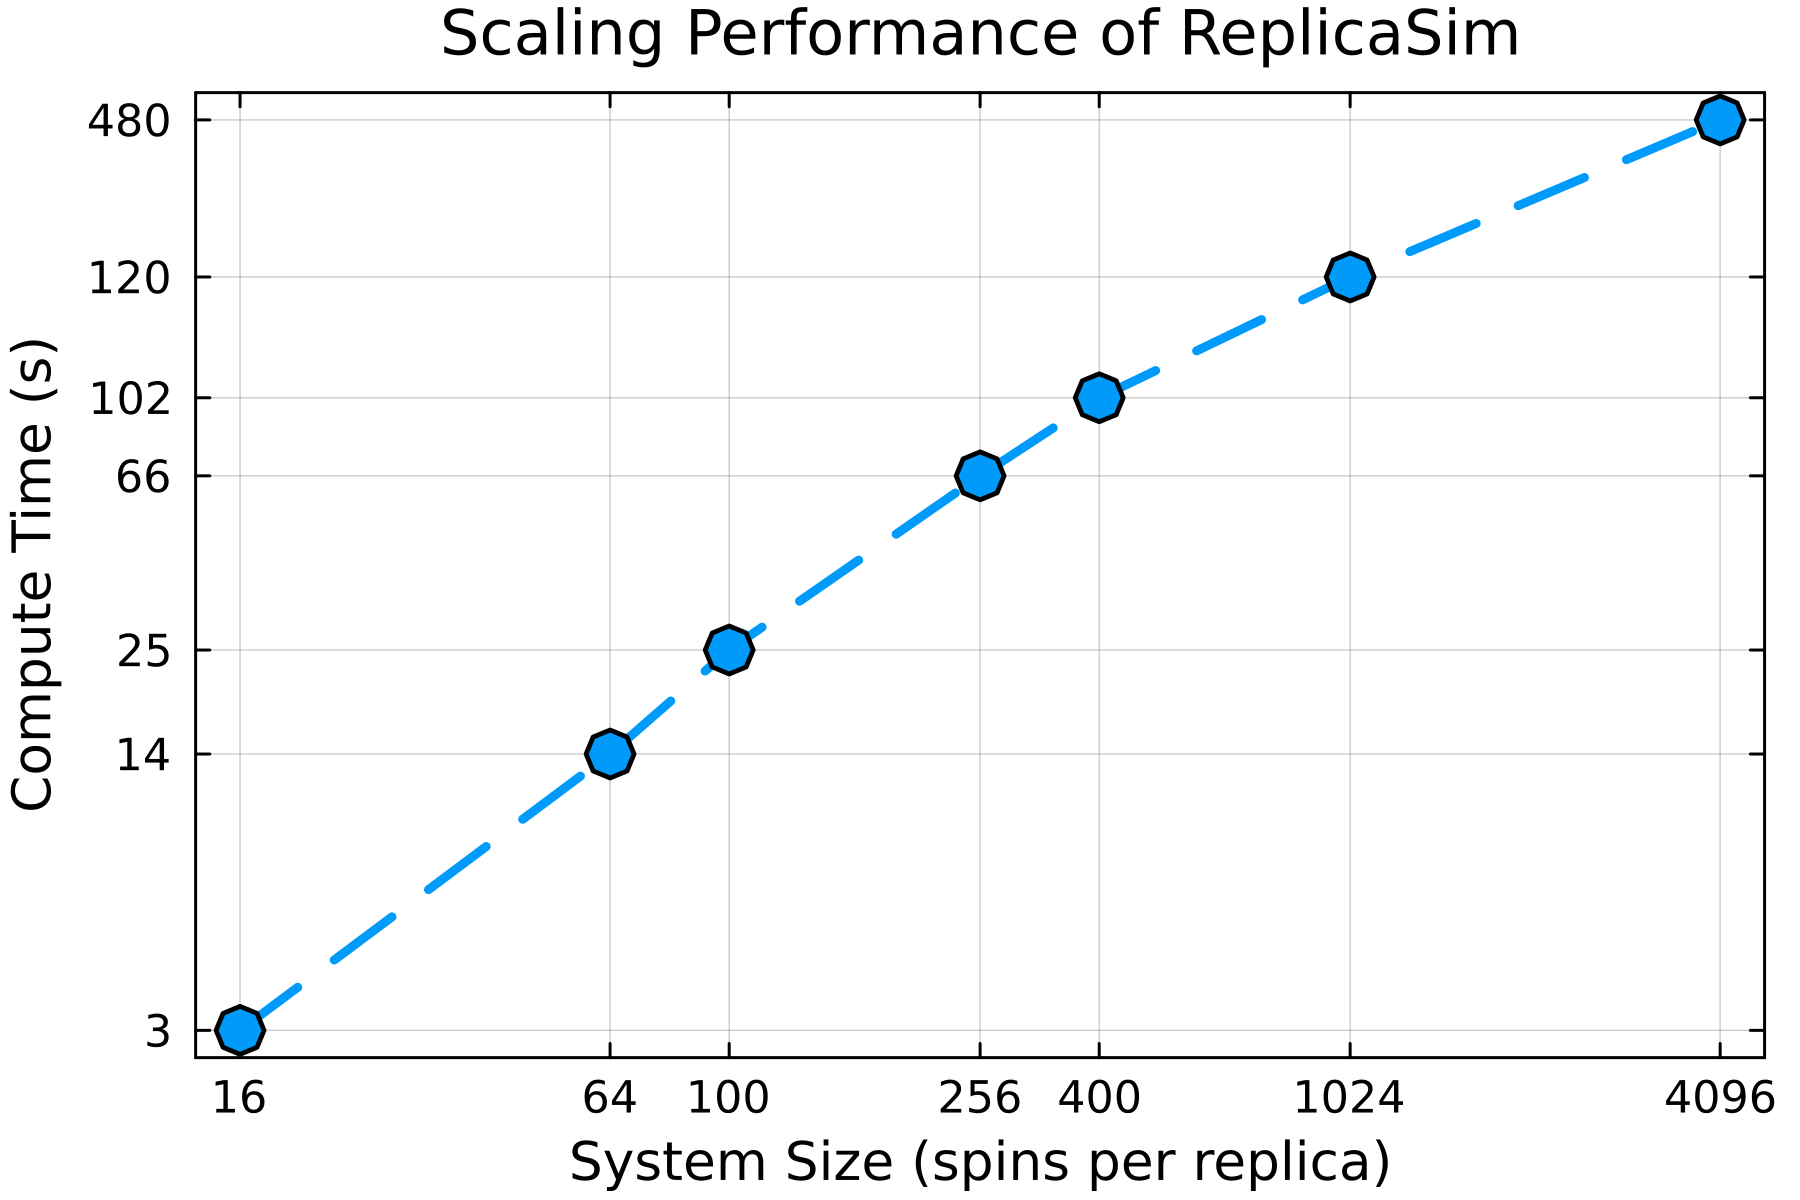
\includegraphics[width=0.95\linewidth]{figures/performance_and_scaling.png}

\caption{Scaling performance of ReplicaSim as a function of system size. The compute time grows with system size, following a scaling behaviour of approximately $O(N)$ scaling compared to $O(N^{2})$ scaling seen in all-to-all dipolar interaction models, indicating a significant efficiency gain. The near-linear scaling is achieved by restricting dipolar interactions to a finite cutoff radius, which limits the number of neighbors considered for each spin, reducing computational complexity.}
 
\end{figure*}
% ==============================================================================

We expect that the runtime can be reduced further by using newer-generation GPUs with higher memory bandwidth and greater parallel processing capabilities. The workload of ReplicaSim is both compute-intensive and memory-intensive: faster global memory access will speed up the neighbour interaction lookups and spin updates, while a larger number of CUDA cores will allow even more operations to be performed simultaneously.

These benchmarking results highlight ReplicaSim’s efficiency for large-scale ASI problems. Complex magnetization dynamics that would be very time-consuming with slower methods become practical to simulate with ReplicaSim, making it a valuable tool for investigating ASI behaviour across a wide range of scales and conditions.

\section{Conclusion}
ReplicaSim was developed to efficiently study artificial spin ice systems at large scales and over long timescales. Traditional micromagnetic simulations solve the Landau-Lifshitz-Gilbert (LLG) equation to track each spin’s real-time evolution. In contrast, Monte Carlo methods use a statistical approach to explore equilibrium and near-equilibrium states without requiring the solution of complex differential equations. Monte Carlo simulations allow us to efficiently study large-scale ASI systems, capturing key collective behaviours like hysteresis and monopole motion in a way that would be computationally prohibitive or inaccessible with micromagnetic solvers.

\section{ReplicaSim: Algorithm Blueprint}

To summarize the core workflow of ReplicaSim, we present the following pseudocode representation:

\begin{algorithm}[h!]
\caption{ReplicaSim: Multi-Replica Parallel Monte Carlo Simulation for ASI}
\label{alg:ReplicaSim}
\begin{algorithmic}[1]
    \State \textbf{Initialize system:}
    \State \quad Define system parameters (lattice size, interaction strengths, temperature)
    \State \quad Generate initial random spin configurations \( S \) and spin magnetization components \( S_X, S_Y \) for all replicas
    \State \quad Precompute neighbor lists and interaction matrices \( J \)
    \State \quad Transfer data to GPU memory

    \For{each external field value \( H \)}
        \For{each Monte Carlo step \( k \)}
            \State \textbf{Perform spin-flip attempts:}
            \For{each replica}
                \State Select a random spin \( i \)
                \State Compute \( \Delta E \) using the dumbbell model and neighbor interactions
                \State Accept or reject the spin flip based on the Metropolis criterion
                \If{flip accepted}
                    \State Update spin state \( S \), magnetization components \( S_X, S_Y \)
                     \State Increment the dumbell energy by  \( \Delta E_{dumbell} \) (if this data is needed; 
                     \State it is not essential for the algorithm, which relies only on spin states 
                     \State and spin components)
                \EndIf
            \EndFor
            \State Compute total magnetization \( M \) across replicas (GPU parallel reduction)
        \EndFor
        \State Record magnetization and energy values
        \If{snapshot condition met}
            \State Save spin configuration
        \EndIf
    \EndFor

    \State \textbf{Output data:}
    \State Store magnetization, energy values, and spin snapshots in JLD2 format
\end{algorithmic}
\end{algorithm}


\bibliography{SASI_MvsH.bib}


\end{document}




